\documentclass{note}
\usepackage[cpp,table]{mypackage}
\usepackage{footnote}
\makesavenoteenv{tabular}

\renewcommand{\thefootnote}{\fnsymbol{footnote}}

\title{数字图像处理笔记}
\author{陈鸿峥}
\date{{\builddatemonth\today}\protect\footnote{\text{Build \builddate\today}}} % protect!

\begin{document}

\maketitle
\renewcommand{\thefootnote}{\arabic{footnote}}
\setcounter{footnote}{0}

\setcounter{tocdepth}{2}%设置深度
\tableofcontents

\bigskip\bigskip

% !TEX root = main.tex

\section{计算机系统概述}
\subsection{计算模型}
\begin{itemize}
	\item 图灵机(1936)
	\item 冯诺依曼体系结构(1945)\footnote{非冯诺依曼体系结构:并行计算、量子计算、生物计算} --- 存储程序原理(\textbf{运算器}为中心)\\
	计算机采用\textbf{二进制}表示机器指令和数据,按照程序指令\textbf{顺序}执行
\begin{center}
\begin{tikzcd}
& & \text{存储器}\arrow{d} & & \\
\quad\arrow{r} & \text{输入设备}\arrow{r} & \text{运算器}\arrow{r}\arrow{d}\arrow{u} & \text{输出设备}\arrow{r} & \quad\\
& & \text{控制器}\arrow{u}\arrow{lu}\arrow{ru}\arrow[bend left]{uu} & &
\end{tikzcd}
\end{center}
而现在由于计算不是瓶颈,存储访问成为了瓶颈,故现代微机以\textbf{存储器}为中心
\begin{center}
\begin{tikzcd}
& & \text{运算器}\arrow{d} & & \\
\quad\arrow{r} & \text{输入设备}\arrow{r} & \text{存储器}\arrow{r}\arrow{d}\arrow{u} & \text{输出设备}\arrow{r} & \quad\\
& & \text{控制器}\arrow{u}\arrow{lu}\arrow{ru}\arrow[bend left]{uu} & &
\end{tikzcd}
\end{center}
\end{itemize}
[运算器、控制器](CPU)、存储器为计算机的核心,合称主机;外围设备,简称外设,指除主机外的其他设备,包括IO设备、外存等

计算机中的信息仍用二进制表示的原因:由物理器件性能决定
\begin{itemize}
	\item 二进制只有两种状态,容易找到具有2个稳定状态并且状态转换容易控制的物理器件(数字电路)
	\item 二进制编码运算规则简单
	\item 二进制的0、1与二值逻辑一致,容易实现逻辑运算
\end{itemize}
% There are two reasons computers use the binary system:
% 1.Two clearly distinct states that provide a safety range for reliability.
% 2.Least amount of necessary circuitry, which results in the least amount of space, energy consumption, and cost.

\subsection{计算机的发展历程}
按发展历程可分为:电子管、晶体管、集成电路、(超)大规模集成电路四代计算机
\par重大历史事件如下
\begin{center}
\begin{tabular}{|c|c|c|c|}
\hline
% 年份 & 姓名 & 事件 & 备注 \\
1904 & 弗莱明(Fleming) & 二极管 & \\\hline
1907 & 德福雷斯特(De Forest) & 三极管 & \\\hline
1938 & 香农(Shannon) & 布尔代数与二值电子器件(继电器) & 奠定数字电路基石 \\\hline
1946 & & 第一台通用计算机ENIAC & 十进制 \\\hline
1947 & \begin{tabular}{c}布莱顿(Brattain)\\
巴丁(Bardeen)\end{tabular} & 点接触晶体管 & \\\hline
1949 & 肖克利(Shockley) & 结型晶体管(1949) & 1956诺贝尔奖\\\hline
1950 & & 二进制和存储程序EDVAC & 实现冯诺依曼设想(组合进步) \\\hline
1958 & Jack Kilby & 集成电路 & 2000诺贝尔奖 \\\hline
1965 & Moore & 摩尔定律 & \begin{tabular}{c}
在价格不变的情况下,每18个月芯片上\\
晶体管数目翻倍,性能也提升一倍
\end{tabular}\\\hline
1971 & Intel & 第一款微处理器4004 & 10$\mu$m\\\hline
\end{tabular}
\end{center}

\subsubsection{单处理器(1971-2002)}
性能提升主要手段
\begin{itemize}
	\item 提升工作主频:KHz增长至GHz(生产工艺进步,流水线级数增加)
	\item 指令级并行(ILP)
\end{itemize}
\begin{proposition}[安迪-比尔定律]
Andy gives, Bill takes away. 安迪是原Intel CEO,比尔是原微软CEO,硬件厂商靠软件开发商用光自己提供的硬件资源得以生存
\end{proposition}
但遇到频率墙和功耗墙
\[\text{功耗(power)}\propto 1/2\times\text{CMOS电容}\times\text{电压}^2\times\text{转换(01)频率}\]
\par
2004年,Intel放弃4GHz Pentium4芯片开发,因无法解决散热问题,通过加快主频提升处理器性能的路走到尽头

\subsubsection{多核处理器(2005-)}
采用多核处理器不过是将硬件的问题丢到软件\footnote{“向多核的转变并不是因为我们在软件或体系结构技术上取得了中大突破而带来的。相反,这种转变是当单处理器体系结构发展遇到了难以克服的巨大障碍时,我们被迫作出的一种选择。”---Kurt Keutzer (UCB), \emph{The Landscape of Parallel Computing Research: A View from Berkeley}}
\begin{theorem}[阿姆达尔(Amdahl)定律]
\label{thm:amdahl}
\[\text{改进后的执行时间}=\text{受改进影响部分的执行时间}/\text{改进提高的倍数}+\text{不受影响的执行时间}\]
\[S_A=\frac{1}{s+(1-s)/N},\]
\end{theorem}
对计算机系统的某个部分采用并行优化措施后所获得的计算机性能的提高是有上限的,上限由串行部分所占的比例决定
\begin{theorem}[古斯塔夫森(Gustafson)定律]
\[S_G=(s'+p'\times N)/(s'+p')=N+(1-N)\times s',\]
其中,$s'$和$p'$为程序串行部分与可并行化部分在并行系统上执行的时间占总时间的比例,$N$为处理器数量,简便起见设总时间$s'+p'=1$
\end{theorem}
打破Amdahl定律\textbf{问题规模不变}的假设,任何足够大的任务都可以被有效地并行化,只要问题规模可扩展,并行所带来的加速比就可以扩展


\subsection{计算机系统的层次结构}
\begin{center}
\begin{tikzcd}
\text{高级语言层}\arrow{d}{}\\
\text{汇编语言层}\arrow{d}{}\\
\text{操作系统层}\arrow{d}{}\\
\text{指令系统层}\arrow{d}{}\\
\text{微体系结构层}\arrow{d}{}\\
\text{数字逻辑层}
\end{tikzcd}
\end{center}
程序编译运行过程:
\begin{center}
\begin{tikzcd}
\text{高级语言}\quad\arrow{r}{\text{预编译、编译}} & \quad\text{汇编语言}\arrow{r}{\text{汇编}} & \text{目标文件(二进制)}\arrow{r}{\text{链接}} & \text{可执行文件(二进制)}\arrow{d}{\text{加载}}\\
& & \text{电路上的电信号}\quad & \quad\text{二进制机器指令流(硬盘$\to$存储器)}\arrow[swap]{l}{\text{CPU取指译码}}
\end{tikzcd}
\end{center}
计算机内部工作过程:逐条执行加载到内存中的二进制机器指令流的过程

指令执行分为两个阶段,周期性重复性进行:
\begin{itemize}
	\item 取指阶段:CPU从内存中读取指令,程序计数器(PC)保存要被要被取出的\textbf{下一条}指令的地址,除非遇跳转指令,否则都加一个增量\footnote{程序计数器(Program Counter)是一个实际存在的寄存器吗? - Belleve的回答 - 知乎 \url{https://www.zhihu.com/question/22609253/answer/21965180} PC每次增加\textbf{一条指令的长度/寻址粒度},在MIPS中一条指令长4字节,寻址粒度1字节,故每次PC加4;而x86体系指令长度不定,每次增加量会变化}
	\item 执行阶段:对取出的指令译码后执行
\end{itemize}
软件系统可分为系统软件和应用软件

\subsection{计算机结构的八个想法}
\begin{enumerate}
	\item 摩尔(Moore)定律:集成电路资源每$18-24$个月翻倍
	\item 抽象(abstraction):简化设计
	\item 加速常用操作(Make common case fast):见定理\ref{thm:amdahl}
	\item 并行(parallelism)
	\item 流水线(pipelining)
	\item 预测(prediction)
	\item 内存等级制(hierarchy)
	\item 冗余实现可靠性(redundancy):检测故障及解决
\end{enumerate}

\subsection{基本指标}
表示计算机通信带宽时
\begin{center}
\begin{tabular}{ccccccc}\hline
KB(yte) & MB & GB & TB & PB & EB & ZB\\\hline
$10^3$ & $10^6$ & $10^9$ & $10^{12}$ & $10^{15}$ & $10^{18}$ & $10^{21}$\\\hline
\end{tabular}
\end{center}
表示计算机存储二进制时
\begin{center}
\begin{tabular}{ccccccc}\hline
KiB(yte) & MiB & GiB & TiB\\\hline
$2^{10}$ & $2^{20}$ & $2^{30}$ & $2^{40}$\\\hline
\end{tabular}
\end{center}
\begin{itemize}
	\item 位(bit/b):计算机处理、存储、传输信息的最小单位
	\item 字节(Byte/B) $1\text{ Byte}=8\text{ bit}$:现代计算机主存按字节编制,字节是最小可寻址单位
	\item 字(Word):表示被处理信息的单位,用来度量数据类型的宽度\footnote{字长是指CPU中\textbf{数据通路的宽度},等于CPU内部总线的宽度或运算器的位数或通用寄存器的宽度;字和字长的宽度可以一样,也可以不同,通常是字节的整数倍}
\end{itemize}
\par 一台32位的电脑,一个字等于4个字节,字长为32位;若字长为16位,则一个字等于2字节.
\par 4字节相当于8位16进制编码

\subsection{性能评价}
\label{subsec:performance}
CPU主频:对同一型号计算机,主频越高,完成指令一个执行步骤时间越短
\[\text{计算机的性能(Performance)}=1/\text{执行时间(Execution time)}\]
按照单位(量纲)进行换算即可
\[\begin{aligned}
\text{CPU执行时间(s)}&=\text{执行程序所需CPU时钟周期(cyc)}\times\text{时钟周期s/cyc)}\\
&=\text{指令数目(ins)}\times\text{CPI(cyc/ins)}\times\text{时钟周期(s/cyc)}
\end{aligned}\]
程序性能对执行事件的影响:
\begin{center}
\begin{tabular}{|c|c|c|c|}\hline
 & 指令数 & CPI & 时钟周期\\\hline
算法、编程语言、编译器 & $\times$ & $\times$ & \\\hline
指令集 & $\times$ & $\times$ & $\times$ \\\hline
计算机组成 & & $\times$ & $\times$ \\\hline
实现技术 & & & $\times$\\\hline
\end{tabular}
\end{center}
体系结构=指令集体系结构(功能定义与设计)+计算机组成(考虑用什么材料)\\
举例来说:
\begin{itemize}
	\item 指令集(ISA)考虑:是否提供乘法指令
	\item 组成(Organization)考虑:如何实现乘法指令(专门乘法器还是加法器+移位器)
	\item 实现技术(Technology)考虑:如何布线、用什么材料和工艺
\end{itemize}

% 带有处理器的设备一般称为智能化设备
% 完整的计算机系统应包括配套的硬件设备和软件系统
% !TEX root = main.tex

\section{空间域图像增强}
图像增强目的是提高图像在特定应用领域的视觉质量,包括光滑、锐化、提取边缘、反转、去噪以及各种滤波等。

空间域图像增强的是直接对图像的像素进行操作,基本关系式可表示如下:
\[g(x,y)=T(f(x,y))\]

\subsection{基本灰度变换}
\begin{itemize}
\item 基本灰度函数:线形、对数、幂次
\begin{figure}[H]
\centering
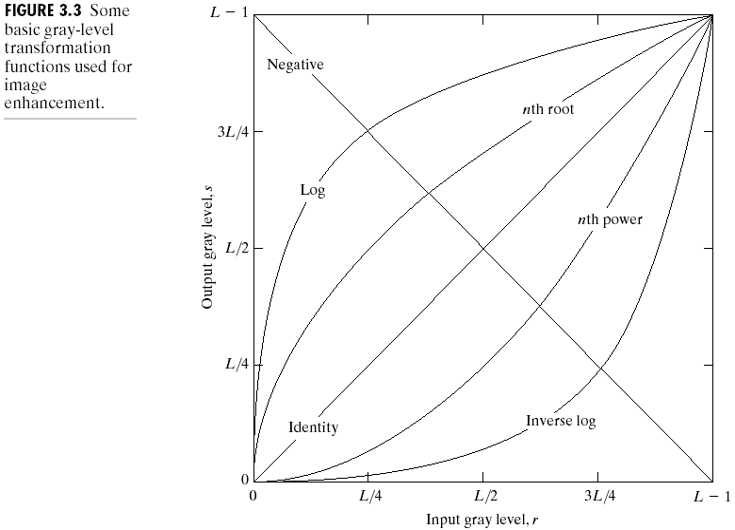
\includegraphics[width=0.6\linewidth]{fig/enhancement.png}
\end{figure}
\item 图像反转变换:$s=L-1-r$,人眼的一个特点就是在背景相对光亮时对灰度层次有较好的分辨能力。
\begin{figure}[H]
\centering
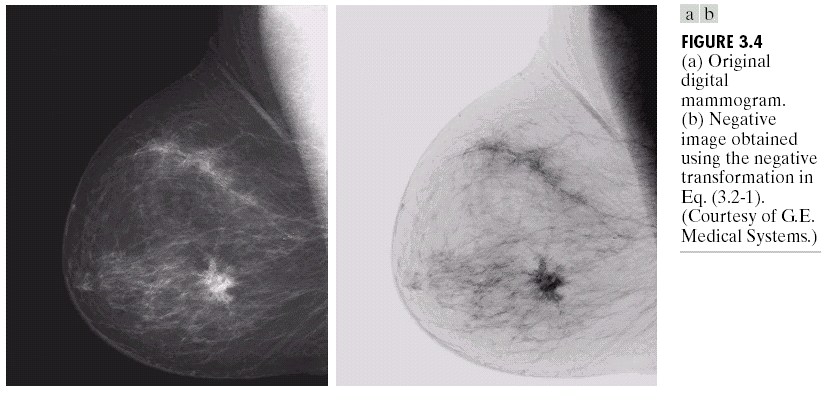
\includegraphics[width=0.6\linewidth]{fig/trans-inverse.png}
\end{figure}
\item 对数变换:$s=c\log(1+r)$,$c$是常数,$r\geq 0$,适合大范围的数据压缩。
任何具有对数函数曲线形状的变换都可以完成灰度的压缩和扩展功能。 
\begin{figure}[H]
\centering
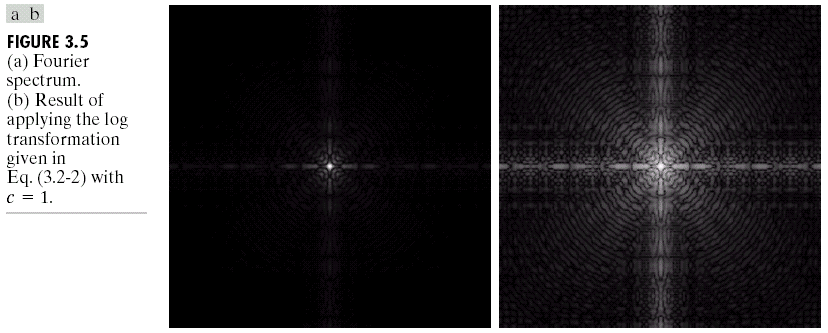
\includegraphics[width=0.6\linewidth]{fig/trans-log.png}
\end{figure}
\item 幂次变换:$s=cr^\gamma$,$c$和$\gamma$都为正常数
\begin{figure}[H]
\centering
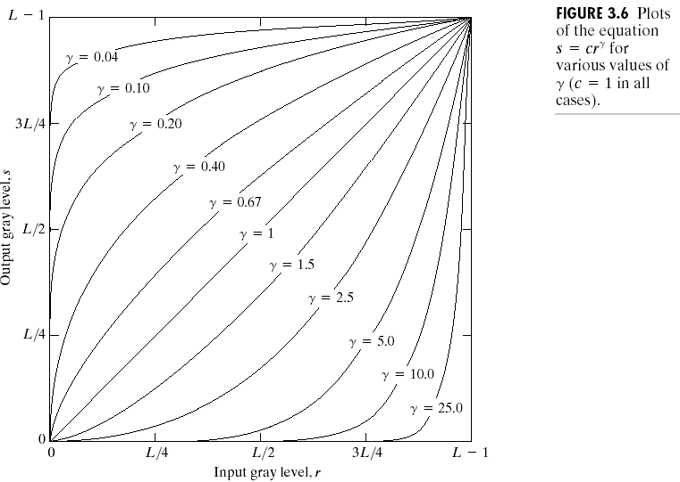
\includegraphics[width=0.6\linewidth]{fig/trans-power.png}
\end{figure}
伽马校正:大量的图像设备如捕捉卡、打印机、数码相机以及显示装置的响应(输出)就对应一个幂函数,通常称这个幂函数的指数为gamma。纠正这个幂次响应的处理称为伽玛校正(gamma correction)。
\begin{figure}[H]
\centering
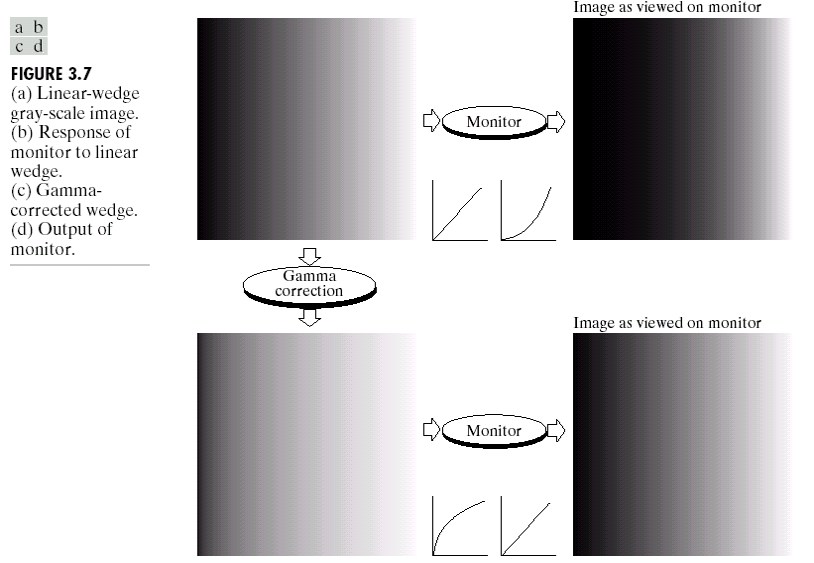
\includegraphics[width=0.6\linewidth]{fig/trans-gamma.png}
\end{figure}
在一般的图像处理软件中,几乎都有伽玛校正的功能。这个功能可用于调整图像的对比度。如果图像偏暗,有些低灰度值的细节被掩盖时,可考虑用指数$\gamma<1$的伽玛校正(变亮);反之,$\gamma>1$的校正对那些被“漂白”的细节会起作用(变暗)。
\item 分段线性变换
\begin{figure}[H]
\centering
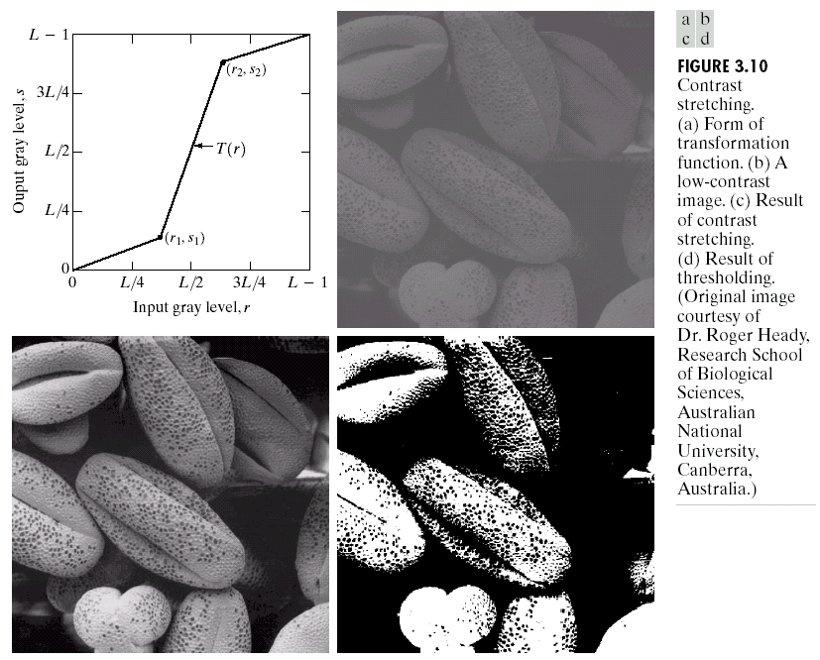
\includegraphics[width=0.6\linewidth]{fig/trans-by-cases.png}
\end{figure}
\item 灰度切割:在图像中提高特定灰度的亮度
\begin{figure}[H]
\centering
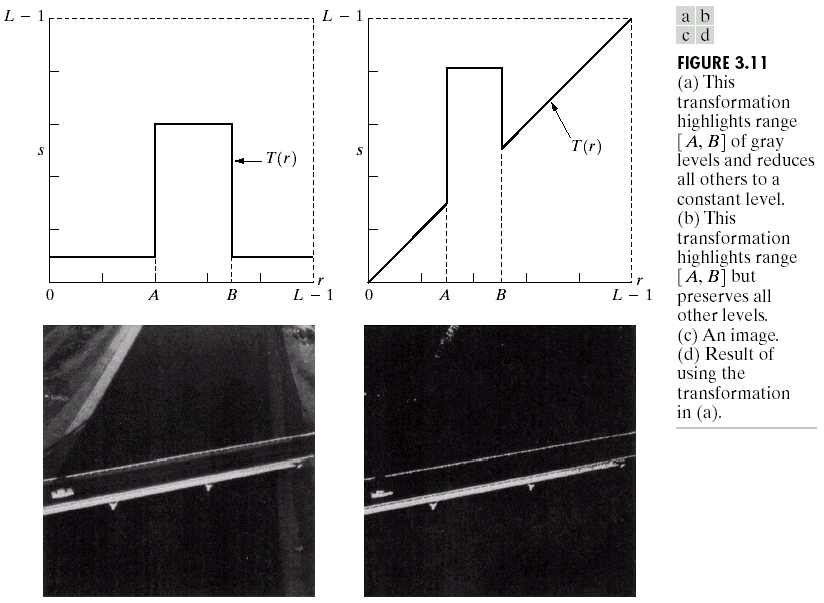
\includegraphics[width=0.6\linewidth]{fig/trans-cut.png}
\end{figure}
\end{itemize}

位图切割:8位灰度图象可以分割成8个位面,每个是一个二值图像(中间切一半)。
\textbf{高位}表示了\textbf{重要的信息},\textbf{低位}给出了\textbf{不同程度的细节}。
\begin{figure}[H]
\centering
\begin{tabular}{cc}
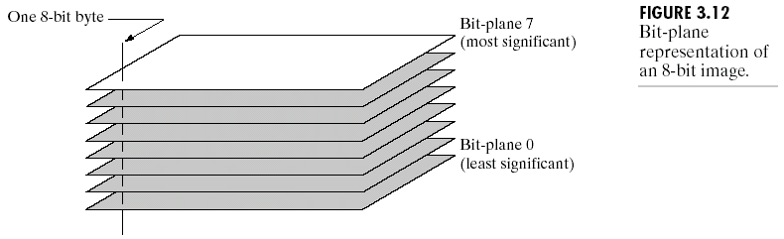
\includegraphics[width=0.5\linewidth]{fig/bitmap.png}&
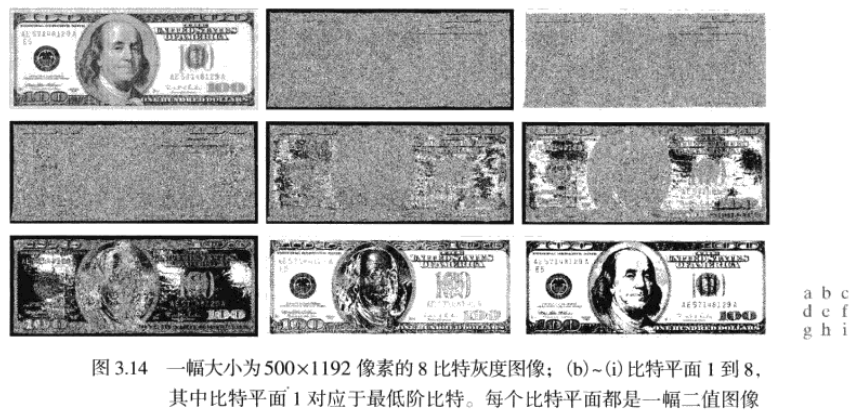
\includegraphics[width=0.5\linewidth]{fig/bitmap-dollars.png}
\end{tabular}
\end{figure}

位图的作用
\begin{itemize}
	\item 信息隐藏:藏在中间位,低位会被丢弃,高位太清楚
	\item 视频传输:先传高位,再传低位,逐渐清晰
\end{itemize}

\subsection{直方图}
\begin{definition}[直方图]
灰度级别为$[0,L-1]$(直方图一定从0开始!)。数字图像直方图是离散函数$h(r_k)=n_k$,其中$r_k$是第$k$级灰度,$n_k$是图像中灰度级为$r_k$的像素个数(频数)。
除以总数$n$就得到归一化的直方图。
\end{definition}

\subsubsection{直方图均衡化}
有亮度差才能看到细节,最好是均衡分布,实现\textbf{高对比度}。
\begin{figure}[H]
\centering
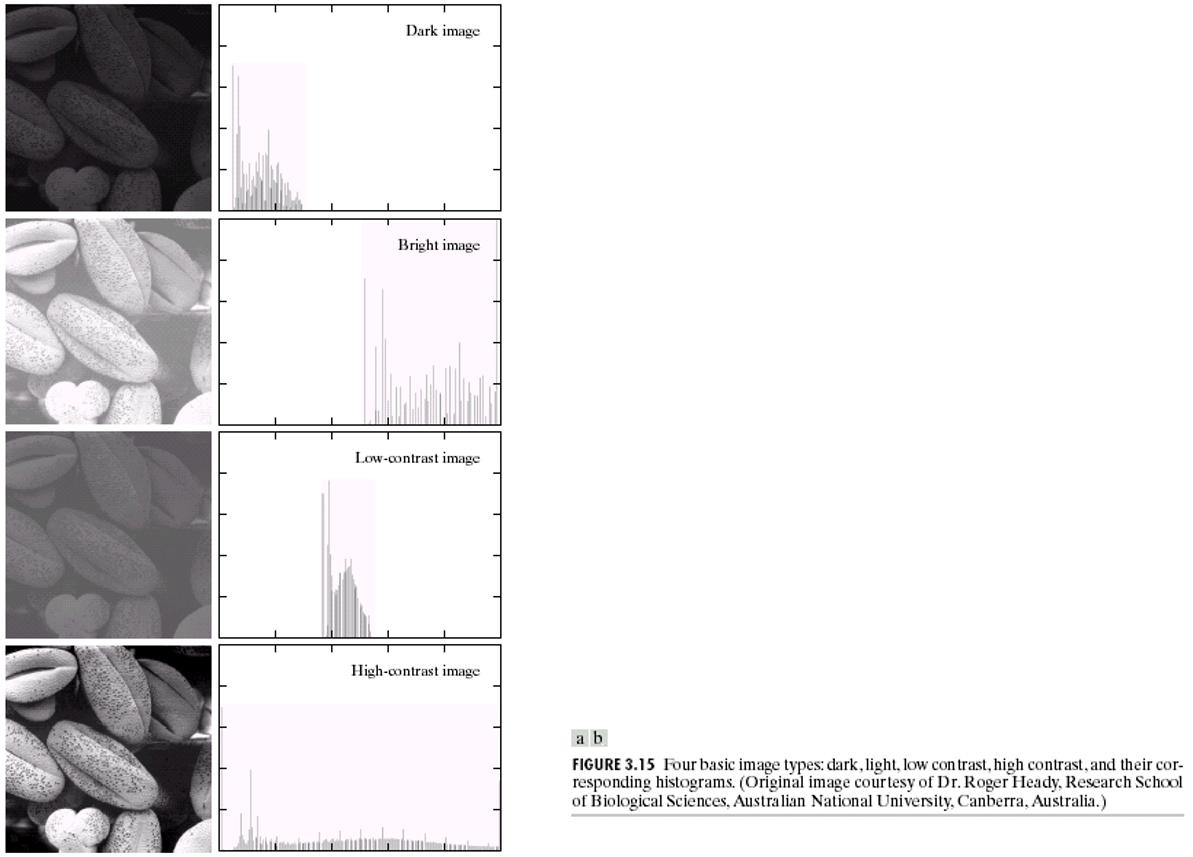
\includegraphics[width=0.6\linewidth]{fig/histogram-quality.png}
\end{figure}

直方图均衡化/线性化则是寻求一种变换使得变换后的图像具有尽可能均匀分布的直方图,用于图像增强最大的特点是自动化,有强大的适应性强的功能。
通常需要满足下列条件:
\begin{itemize}
	\item $T(r)$在$0\leq r\leq L-1$中为单值且单调递增
	\item 当$0\leq r\leq L-1$时,$0\leq T(r)\leq L-1$
\end{itemize}
步骤如下:
\begin{enumerate}
	\item 概率$p_r(r_k)=n_k/n,k=0,1,2,\ldots,L-1$
	\item 累计分布函数(PDF)
	\[P(r_k)=\sum_{j=0}^k p_r(r_j)=\sum_{j=0}^k\frac{n_j}{n},k=0,1,2,\ldots,L-1\]
	\item 变换函数
	\[s_k=T(r_k)=(L-1)\cdot\sum_{j=0}^k\frac{n_j}{n},k=0,1,2,\ldots,L-1\]
	\item 将$s_k$四舍五入转换为标准灰度级别,如有相同$\lceil s_k\rceil$则合并
\end{enumerate}
\begin{figure}[H]
\centering
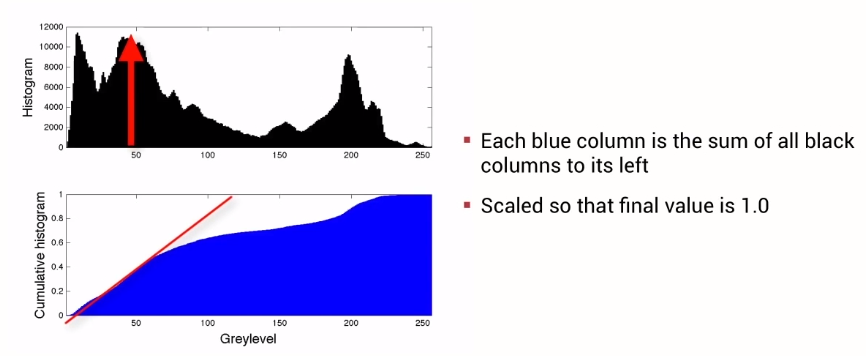
\includegraphics[width=0.8\linewidth]{fig/histogram-normalization.png}
\end{figure}
\begin{analysis}
若$r$为离散型随机变量,$T(r)$为单调递增函数($T^{-1}$存在且单调),且$s=T(r)$,则由概率论有
\[p_s(s)=p_r(r)\pd{r}{s}\Big|_{r=T^{-1}(s)}=p_s(T^{-1}(s))|T^{-1}(s)|\]
考虑变换函数为$r$的累积分布函数(CDF)
\[s=T(r)=\intabu{0}{r}{p_r(\omega)}{\omega}\]
对$s$求导并代入上面的式子可得$p_s(s)=1$,故实现均衡。
算法实际上就是求累积分布函数,使得原本亮度小的像素能够映射到亮度大的空间。
\end{analysis}

\subsubsection{直方图匹配}
当两幅图像比对时,通常要使其直方图形式一致(如不同光照条件下的同一场景)。
先是做空间归一化(伸缩、旋转),然后再做像素的归一化。

做法是使两幅图像均衡化后的结果相同,即
\[\begin{aligned}
s&=T(r)=\intabu{0}{r}{p_r(w)}{w}\\
s&=G(z)=\intabu{0}{z}{p_z(t)}{t}\\
\implies z&=G^{-1}(s)=G^{-1}(T(r))
\end{aligned}\]

具体步骤如下:
\begin{enumerate}
	\item 计算出原图的直方图
	\[s_k=T(r_k)=(L-1)\sum_{j=0}^k\frac{n_j}{n}\]
	\item 给出输出图像期望的直方图$p_z(z)$,并令
	\[v_k=G(z_k)=(L-1)\sum_{i=0}^kp_z(z_i)=s_k\]
	\item 寻找区间$[0,L-1]$的最小整数$\hat{z}$,使得
	\[G(\hat{z})-s_k\geq 0\]
	即由$k$映射到$\hat{z}$
\end{enumerate}

\begin{definition}[$n$阶矩]
设$p_r(r_k)=n_k/n$,则$r$的第$n$阶中心矩为
\[\mu_r(r_k)=\sum_{i=0}^{L-1}(r_i-\bar{r})^np(r_k)\]
其中$\bar{r}=\sum_{i=1}^{L-1}r_ip(r_i)$为$r$的平均值。
特别地,当$n=2$时为方差。
\end{definition}


\subsection{空间滤波基础}
滤波的概念来自信号处理中的傅里叶变换,空间滤波指的是直接对图像像素进行处理的操作。
滤波器(filter)有时也叫掩模(mask)、核(kernel)、模板(template)或窗口(window)。

\subsubsection{线性滤波}
空间域线性滤波基本公式:
\[g(x,y)=\sum_{s=-a}^a\sum_{t=-b}^b w(s,t)f(x+s,y+t)\]
常见的情况是,$a=b$为奇数,如1、3、5。

\begin{definition}[相关与卷积]
一个$m\times n$的滤波器$w(x,y)$与$M\times N$图像$f(x,y)$的相关操作定义为
\[w(x,y)\circ f(x,y)=\sum_{s=-a}^a\sum_{t=-b}^b w(s,t)f(x+s,y+t)\]
一个$m\times n$的滤波器$w(x,y)$与$M\times N$图像$f(x,y)$的卷积定义为
\[w(x,y)*f(x,y)=\sum_{s=-a}^a\sum_{t=-b}^b w(s,t)f(x-s,y-t)\]
其中右侧等号表示将$f$旋转$180\degree$(或先沿$x$轴翻折,再沿$y$轴翻折)
\end{definition}
\begin{figure}[H]
\centering
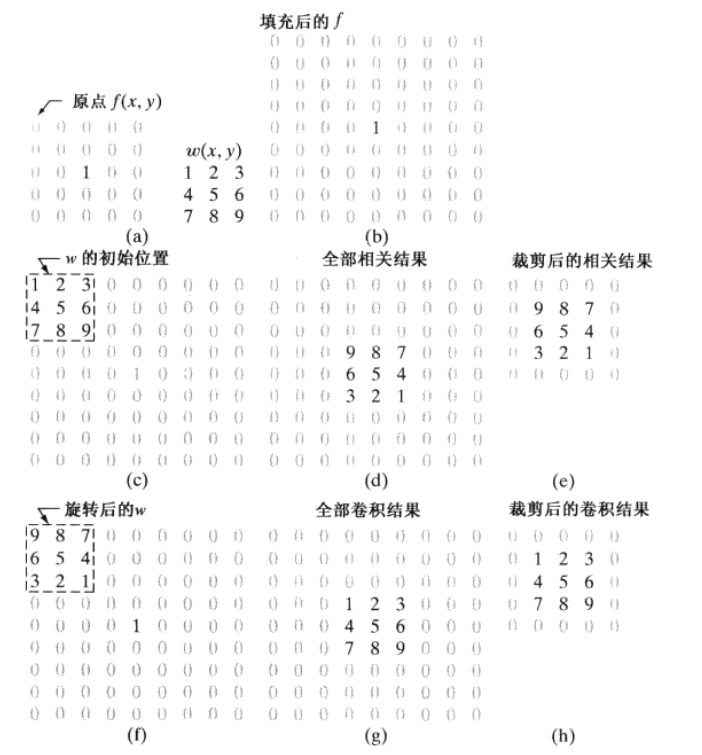
\includegraphics[width=0.5\linewidth]{fig/convolution_and_correlation.png}
\end{figure}

空间滤波对边界的处理方法
\begin{itemize}
	\item 重复边缘值
	\item 卷绕输入图像
	\item 补零(最常用)
	\item 勿略
\end{itemize}

常用的平滑滤波器(左侧是均值滤波)
\[g(x,y)=\frac{\disp\sum_{s=-a}^a\sum_{t=-b}^b w(s,t)f(x+s,y+t)}{\disp\sum_{s=-a}^a\sum_{t=-b}^b w(s,t)}\]
\begin{center}
\begin{tabular}{|c|c|c||c|c|c|}\hline
1/9 & 1/9 & 1/9 & 1/16 & 1/8 & 1/16\\\hline
1/9 & 1/9 & 1/9 & 1/8 & 1/4 & 1/8 \\\hline
1/9 & 1/9 & 1/9 & 1/16 & 1/8 & 1/16\\\hline
\end{tabular}
\end{center}

\subsubsection{非线性滤波}
排序统计滤波器是一种非线性的、 非卷积滤波器。
排序统计滤波器在滤波器包围的像素范围内排序,然后由统计排序结果决定的值代替中心像素的值。
按排序输出的位置分,可分为:中值滤波、最大值滤波、最小值滤波。

中值滤波比均值滤波更适合做\textbf{椒盐噪声}\footnote{特别大或特别小的噪声}的去除,因为噪声总是最大最小,故做中值滤波容易去除。
\begin{figure}[H]
\centering
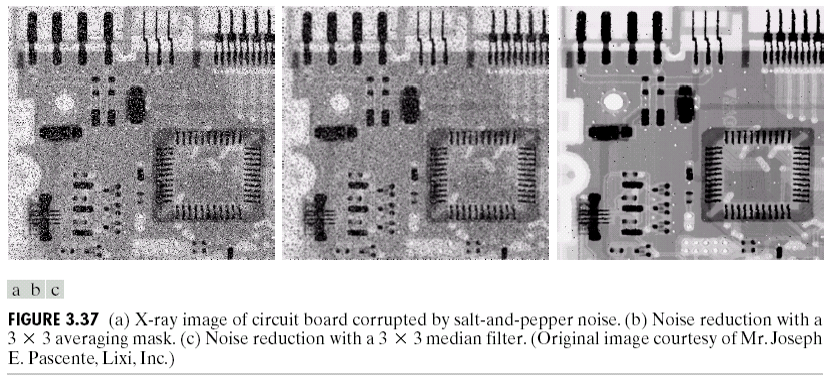
\includegraphics[width=0.8\linewidth]{fig/salt-and-pepper-noise.png}
\end{figure}

同理除了中值滤波,也可以构造第$X$百分点的滤波器。
通常$X<50$图像趋于变暗,$X>50$图像趋于变亮。


\subsection{图像锐化}
\subsubsection{图像微分}
\textbf{积分运算可以做平滑,微分运算可以做锐化!}
锐化的目的即突出图像中的细节或者增强被模糊的细节。

考虑离散情况
\[\begin{cases}
\pd{f}{x}&=f(x+1)-f(x)\\
\pdd{f}{x}&=f(x+1)+f(x-1)-2f(x)
\end{cases}\]

斜边缘、$\delta$/冲击边缘、阶梯边缘
\begin{figure}[H]
\centering
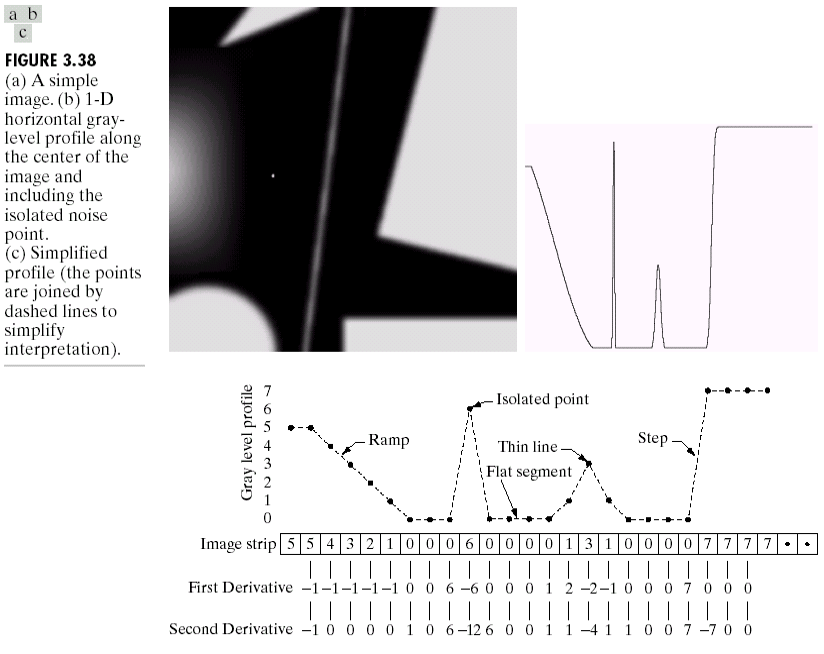
\includegraphics[width=0.6\linewidth]{fig/differential.png}
\end{figure}
\begin{itemize}
\item 一阶微分产生较“宽”的边界,二阶微分产生较“细”的边界
\item 二阶微分处理对细节有较强的响应,如细线和孤立点
\item 一阶微分对阶梯状的灰度变化有较强的响应
\item 二阶微分在处理阶梯状灰度变化时产生双响应
\item 如果灰度的变化相似,二阶微分对线的反应比对阶梯强,对点的反应比对线强
\end{itemize}

\subsubsection{拉普拉斯算子}
\begin{definition}[拉普拉斯(Laplacian)算子]
对连续函数情形,最简单且各向同性的二阶微分算子是拉普拉斯算子
\[\nabla^2 f=\pdd{f}{x}+\pdd{f}{y}\]
离散情况
\[\nabla^2=f(x+1,y)+f(x-1,y)+f(x,y+1)+f(x,y-1)-4f(x,y)\]
\end{definition}
拉普拉斯变换目的是\textbf{获得细节},加回原图像才能进行锐化。
\begin{figure}[H]
\centering
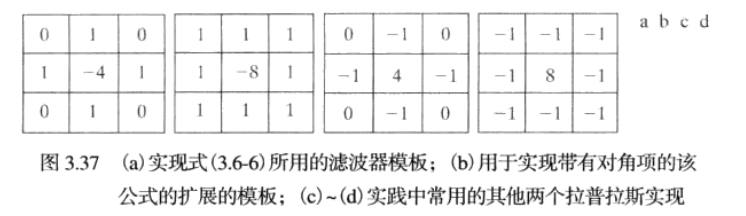
\includegraphics[width=0.6\linewidth]{fig/laplacian_mask.png}
\end{figure}

其实直接从滤波器的表示也可以直观看出这种滤波对图像的突变有比较强的响应(即在突变的位置有较大的输出值),对灰度变化缓慢的区域滤波响应的值会变得很小(变暗)。因此,用拉普拉斯算子作用后,产生的图像将是在暗背景上的一些灰色边线和一些突变点。若将原始图像叠加到拉普拉斯变换后的图像,既可以保护拉普拉斯锐化处理的效果,同时又能复原背景信息。 
拉普拉斯图像增强基本方法:
\[g(x,y)=\begin{cases}
f(x,y)-\nabla^2f & \text{拉普拉斯滤波中心系数为负}\\
f(x,y)+\nabla^2f & \text{拉普拉斯滤波中心系数为正}
\end{cases}\]
\begin{figure}[H]
\centering
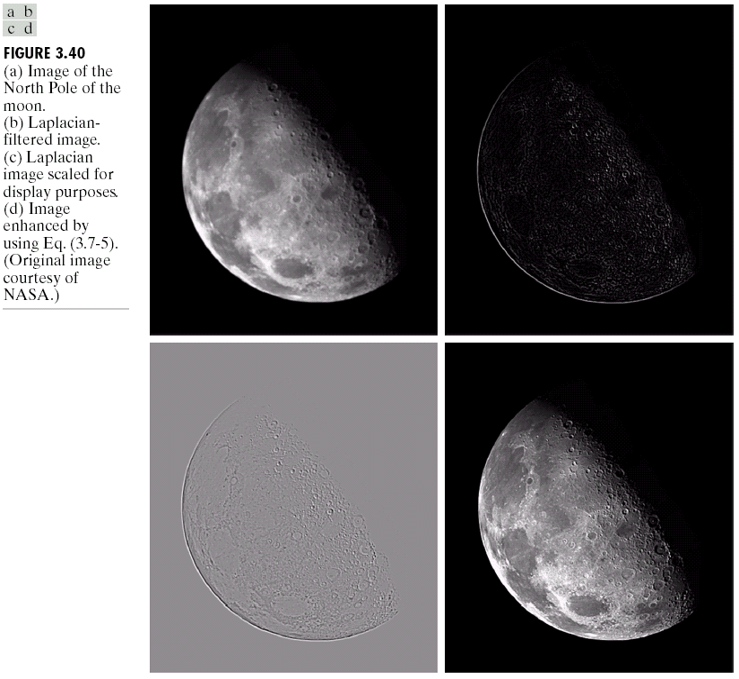
\includegraphics[width=0.6\linewidth]{fig/Laplacian.png}
\end{figure}

\begin{definition}[反锐化掩膜(unsharp masking)]
把原图的一个模糊过的图像从原图中减去,从而得到一个相对清晰的图像
\[f_s(x,y)=f(x,y)-\bar{f}(x,y)\]
就像一个模糊的负片和一个正片放在一起冲洗出相对清晰的照片
\end{definition}
\begin{definition}[高提升滤波(high-boost filtering)]
添加一个系数项$A$得到
\[f_{hb}(x,y)=Af(x,y)-\bar{f}(x,y)=(A-1)f(x,y)+f_s(x,y)\]
其中$A\geq 1$,目的为提升原图亮度,前一部分调整了原图的灰度,后一部分是锐化过的图像。
$A$越大则细节越不清晰,因为原图变亮了。
\end{definition}

可以得到基于拉普拉斯算子的高提升滤波
\[f_{hb}(x,y)=
\begin{cases}
Af(x,y)-\nabla^2 f & \text{Laplacian中心系数为负}\\
Af(x,y)+\nabla^2 f & \text{Laplacian中心系数为正}
\end{cases}\]
当$A=1$时就是拉普拉斯图像增强方法,当$A$足够大时,锐化效果将变得不明显。
\begin{figure}[H]
\centering
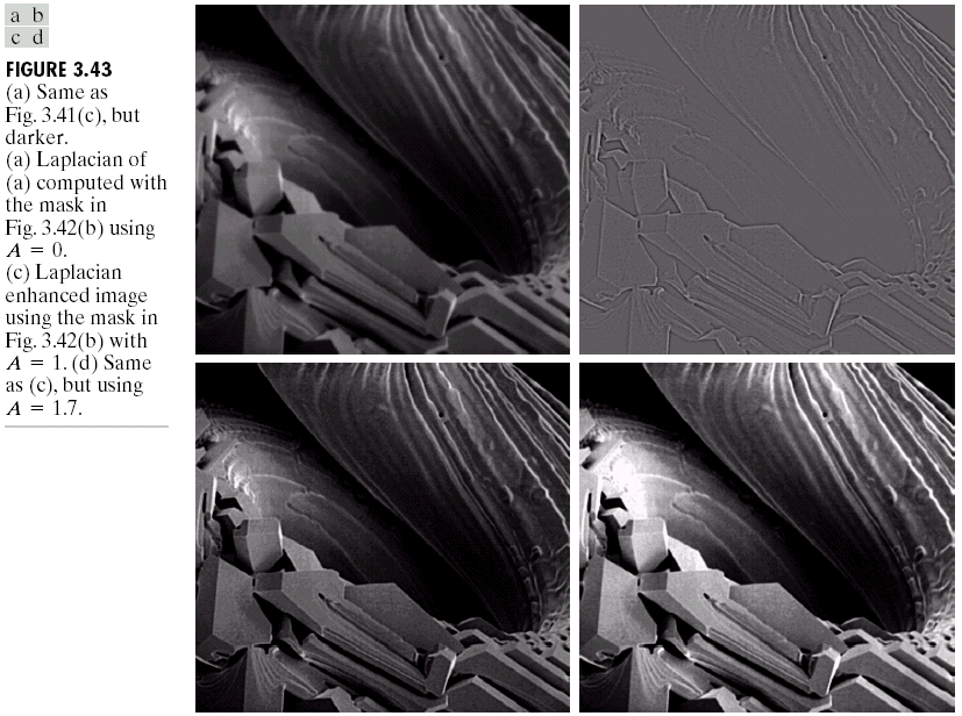
\includegraphics[width=0.6\linewidth]{fig/high-boost.png}
\end{figure}

\subsubsection{梯度}
一阶微分在灰度的跳跃性间断处(边界处)有较强的响应,所以在一些情况下也可以用于图像增强,常用作\textbf{边缘检测}。
考虑二维函数的梯度
\[\nabla\vf=\bmat{G_x & G_y}=\bmat{\pd{f}{x} & \pd{f}{y}}\]
定义$L_2$范数/模
\[\nabla f=(G_x^2+G_y^2)^{1/2}=\lrp{\lrp{\pd{f}{x}}^2+\lrp{\pd{f}{x}}^2}^{1/2}\]
$L_2$模具有各向同性的性质,但计算不方便,故常用$L_1$范数做代替
\[\nabla f\approx |G_x|+|G_y|\]
注意:通常在不引起混淆的情况下,把梯度的模称为梯度。
\begin{itemize}
\item Robert交叉梯度算子
\[\nabla f=|z_9-z_5|+|z_8-z_6|\]
\item Sobel算子:水平边缘增强
\[\nabla f=|(z_7+2z_8+z_9)-(z_1+2z_2+z_3)|+|(z_3+2z_6+z_9)-(z_1+2z_4+z_7)|\]
\begin{figure}[H]
\centering
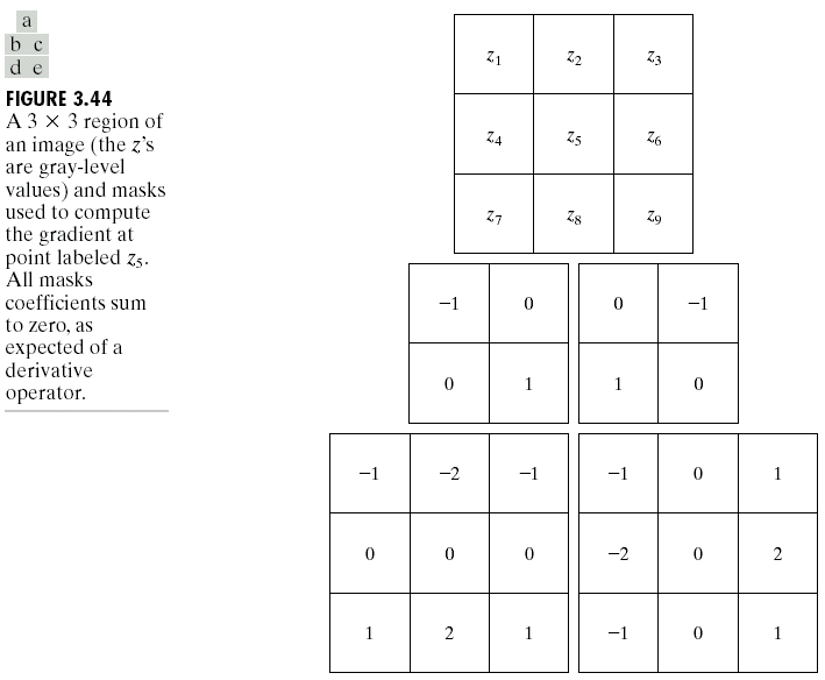
\includegraphics[width=0.4\linewidth]{fig/sobel_and_robert.png}
\end{figure}
\end{itemize}

通常实际使用时是多种滤波器混合使用。
下列为Matlab中预定义的滤波器。
\begin{itemize}
\item Gaussian 低通滤波器
\item Sobel 水平边缘增强滤波器
\item Prewitt 水平边缘增强滤波器:将Sobel的系数绝对值全改为1
\item Laplacian 近似二维拉普拉斯运算滤波器
\item Log (Laplacian of Gaussian)高斯拉普拉斯滤波器
\item Average 均值滤波器
\item Unsharp 模糊对比增强滤波器
\end{itemize}
% !TEX root = main.tex

\section{频率域滤波}
\subsection{傅里叶级数与傅里叶变换}
\begin{definition}[傅里叶级数]
设$f(t)$为以$T$为周期的函数,绝对可积,则$f(t)$可表示为
\[f(t)=\sum_{n=-\infty}^{\infty}c_n\ee^{j\frac{2\pi n}{T}t}\]
其中$j$为虚数单位,
\[c_n=\frac{1}{T}\intabu{-T/2}{T/2}{f(t)\ee^{-j\frac{2\pi n}{T}t}}{t},\,n=0,\pm 1,\pm 2,\ldots\]
\end{definition}

傅里叶级数中每一个基函数都是一个单频谐波,对应的系数/频谱表明原函数对这种频率成分贡献的大小(原函数在这个谐波上的投影)

\begin{definition}[冲激/狄利克$\delta$函数]
面积为1的长方形不断压扁,最后变成宽为0,高为无穷大的函数(左侧为连续情况,右侧为离散情况)
\[\delta(t)=\begin{cases}
\infty & t=0\\
0 & t\ne 0
\end{cases}\qquad
\delta(x)=\begin{cases}
1 & x=0\\
0 & x\ne 0
\end{cases}\]
即
\[\intab{-\infty}{\infty}{\delta(t)}=1
\qquad
\sum_{x=-\infty}^{\infty}\delta(x)=1\]
具有取样(sifting)特性
\[\intab{-\infty}{\infty}{f(t)\delta(t-t_0)}=f(t_0)
\qquad
\sum_{x=-\infty}^{\infty}f(x)\delta(x-x_0)=f(x_0)\]
\end{definition}
\begin{definition}[冲激串]
无限多个分离的周期冲激单元$\Delta T$之和
\[s_{\Delta T}(t)=\sum_{n=-\infty}^{\infty}\delta(t-n\Delta T)\]
\end{definition}
\begin{figure}[H]
\centering
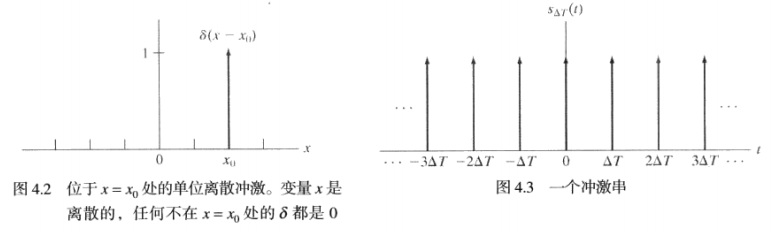
\includegraphics[width=0.8\linewidth]{fig/impulse.png}
\end{figure}

\begin{definition}[傅里叶变换与反变换]
连续情形的傅里叶变换(函数投影,取负号得共轭)和反变换为
\[\begin{aligned}
F(u)&=\Im[f(t)]=\intabu{-\infty}{+\infty}{f(t)\ee^{-j 2\pi ut}}{t}\\
f(t)&=\Im^{-1}[F(u)]=\intabu{-\infty}{+\infty}{F(u)\ee^{j 2\pi ut}}{u}
\end{aligned}\]
这两者构成一个傅里叶变换对。
对于离散情形有
\[\begin{aligned}
F(u)&=\sum_{x=0}^{M-1}f(x)\ee^{-j2\pi ux/M}\\
f(x)&=\frac{1}{M}\sum_{u=0}^{M-1}F(u)\ee^{j2\pi ux/M}
\end{aligned}\]
\end{definition}
由于傅里叶变换是$f(t)$乘上正弦项的展开,正弦项的频率由$\mu$决定(变量$t$已经被积分),积分后只剩下频率,故称傅里叶变换域是频率域。
注意坐标轴已经变化了,现在\textbf{横轴为频率}。

\begin{example}
矩形函数
\[f(t)=\begin{cases}
A & -W/2\leq t\leq W/2\\
0 & \text{otherwise}
\end{cases}\]
的傅里叶变换为
\[\begin{aligned}
F(u)&=\intabu{-W/2}{W/2}{A\ee^{-j2\pi ut}}{t}\\
&=\frac{-A}{j2\pi\mu}[\ee^{-j2\pi\mu W}-\ee^{j2\pi\mu W}]\\
&=AW\frac{\sin(\pi\mu W)}{\pi\mu W}=AW\sinc(\mu W)
\end{aligned}\]
\end{example}
\begin{example}
冲激的傅里叶变换(由取样特性)
\[F(\mu)=\intabu{-\infty}{\infty}{\delta(t)\ee^{-j2\pi\mu t}}{t}=\ee^{-j2\pi\mu 0}=1\]
而位于$t=t_0$的冲激傅里叶变换为
\[F(\mu)=\intabu{-\infty}{\infty}{\delta(t-t_0)\ee^{-j2\pi\mu t}}{t}=\ee^{-j2\pi\mu t_0}\]
周期冲激串的傅里叶变换
\[S(\mu)=\Im[s_{\Delta T}(t)]=\frac{1}{\Delta T}\sum_{n=-\infty}^{\infty}\delta\lrp{\mu-\frac{n}{\Delta T}}\]
\end{example}

\begin{definition}[卷积]
连续情形有
\[f(t)*h(t)=\intabu{-\infty}{+\infty}{f(\tau)h(t-\tau)}{\tau}\]
离散情形有
\[f(x)*h(x)=\sum_{m=0}^{M-1}f(m)h(x-m)\]
\end{definition}
\begin{theorem}[卷积定理]
建立起空间域和频率域\footnote{$t$所在的域称为空间域,$\mu$所在的域称为频率域}的联系
\[f(t)*h(t)\iff F(\mu)H(\mu)
\qquad
f(t)h(t)\iff F(\mu)*H(\mu)\]
即空间域两个函数卷积的傅里叶变换等于两个函数的傅里叶变换在频率域的乘积
\end{theorem}
\begin{analysis}
\[\begin{aligned}
\Im[f(t)*h(t)]&=\intabu{-\infty}{\infty}{\lrs{\intabu{-\infty}{\infty}{f(\tau)h(t-\tau)}{\tau}}\ee^{-j2\pi\mu t}}{t}\\
&=\intabu{-\infty}{\infty}{f(\tau)\lrs{\intabu{-\infty}{\infty}{h(t-\tau)\ee^{-j2\pi\mu t}}{t}}}{\tau}\\
&=\intabu{-\infty}{\infty}{f(\tau)\lrs{H(\mu)\ee^{-j2\pi\mu\tau}}}{\tau}\\
&=H(\mu)\intabu{-\infty}{\infty}{f(\tau)\lrs{\ee^{-j2\pi\mu\tau}}}{\tau}\\
&=H(\mu)F(\mu)
\end{aligned}\]
\end{analysis}

\subsection{取样函数}
\begin{example}
求取样函数
\[\tilde{f}(t)=f(t)s_{\Delta T}(t)=\sum_{n=-\infty}^{\infty}f(t)\delta(t-n\Delta T)\]
的傅里叶变换
\end{example}
\begin{analysis}
由卷积定理
\[\begin{aligned}
\tilde{F}(u)&=\Im[\tilde{f}(t)]=\Im[f(t)s_{\Delta T}(t)]\\
&=F(u)*S(u)=\intabu{-\infty}{\infty}{F(\tau)S(u-\tau)}{\tau}\\
&=\frac{1}{\Delta T}\intabu{-\infty}{\infty}{F(\tau)\sum_{n=-\infty}^{\infty}\delta\lrp{u-\tau-\frac{n}{\Delta T}}}{\tau}\\
&=\frac{1}{\Delta T}\sum_{n=-\infty}^{\infty}F\lrp{u-\frac{n}{\Delta T}}
\end{aligned}\]
\end{analysis}

\begin{theorem}[奈奎斯特(Nyquist)采样定理]
如果以超过函数最高频率的两倍的采样率来获得样本,则连续的带限函数\footnote{对于以原点为中心的有限区间(带宽)之外的频率值,其傅里叶变换为零。
}可以完全从它的样本集恢复,即
\[\frac{1}{\Delta T}>2\mu_{\max}\]
\end{theorem}

若以低于两倍的采样率来采样则会出现混淆现象
\begin{figure}[H]
\centering
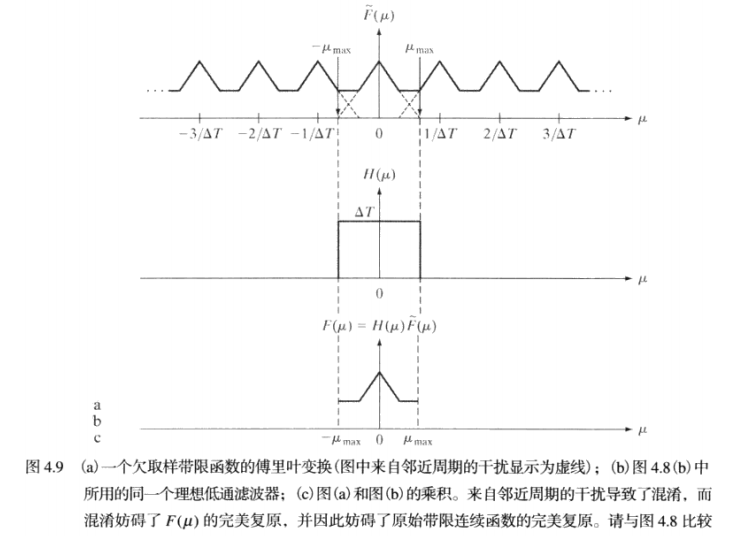
\includegraphics[width=0.8\linewidth]{fig/nyquist.png}
\end{figure}

由取样数据重建函数
\[f(t)=\sum_{n=-\infty}^{\infty}f(n\Delta T)\sinc\lrs{\frac{t-n\Delta T}{\Delta T}}\]

\subsection{二维傅里叶变换}
\begin{definition}[二维冲激]
\[\delta(t,z)=\begin{cases}
\infty & t=z=0\\
0 & \text{otherwise}
\end{cases}\qquad
\delta(x,y)=\begin{cases}
1 & x=y=0\\
0 & \text{otherwise}
\end{cases}\]
有取样特性
\[\sum_{x=-\infty}^\infty\sum_{y=-\infty}^\infty f(x,y)\delta(x-x_0,y-y_0)=f(x_0,y_0)\]
\end{definition}
\begin{definition}[二维离散傅里叶变换]
二维连续傅里叶变换对
\[\begin{aligned}
F(u,v)&=\intabu{-\infty}{\infty}{\intabu{-\infty}{\infty}{f(t,z)\ee^{-j2\pi(ut+vz)}}{t}}{z}\\
f(t,z)&=\intabu{-\infty}{\infty}{\intabu{-\infty}{\infty}{F(u,v)\ee^{j2\pi(ut+vz)}}{u}}{v}
\end{aligned}\]
二维离散傅里叶变换对
\[\begin{aligned}
F(u,v)&=\sum_{x=0}^{M-1}\sum_{y=0}^{N-1}f(x,y)\ee^{-2j\pi (ux/M+vy/N)}\\
f(x,y)&=\frac{1}{MN}\sum_{u=0}^{M-1}\sum_{v=0}^{N-1}F(u,v)\ee^{2\pi j(ux/M+vy/N)}
\end{aligned}\]
\end{definition}
\begin{theorem}[二维采样定理]
二维取样基于二维冲激串
\[\tilde{f}(t,z)=f(t,z)s_{\Delta T\Delta Z}(t,z)=\sum_{m=-\infty}^{\infty}\sum_{n=-\infty}^{\infty}f(t,z)\delta(t-m\Delta T,z-n\Delta Z)\]
取样率需要满足
\[\frac{1}{\Delta T}>2\mu_{\max}\qquad\frac{1}{\Delta Z}>2v_{\max}\]
\end{theorem}
\begin{definition}[傅里叶谱和相角]
由于二维DFT通常为复函数,因此用极坐标形式表示
\[F(u,v)=|F(u,v)|\ee^{j\varphi(u,v)}\]
其中幅度
\[|F(u,v)|=\sqrt{\Real^2(u,v)+\Imag^2(u,v)}\]
称为傅里叶谱,而
\[\varphi(u,v)=\arctan\lrs{\frac{\Imag(u,v)}{\Real(u,v)}}\]
为相角,
\[P(u,v)=|F(u,v)|^2\]
为功率谱
\end{definition}

注意$F(u,v)$的大小只是代表某一频率分量的数目,类似于直方图的概念。
频率域的坐标轴为$u,v$,因此中心点为$(0,0)$,
\[F(0,0)=\sum_{x=0}^{M-1}\sum_{y=0}^{N-1}f(x,y)=MN\bar{f}(x,y)\]
为图像的平均灰度。
即$u$方向和$v$方向上最低频的位置,零点处两个方向的频率都为零,因此这个量经常也被称为频谱的直流分量(DC)。

\begin{example}[陷波滤波器(notch filter)]
使得处理后的图像均值为0,从而使图像的整体灰度降低
\[H(u,v)=\begin{cases}
0 & (u,v)=(M/2,N/2)\\
1 & \text{others}
\end{cases}\]
\end{example}

\begin{figure}[H]
\centering
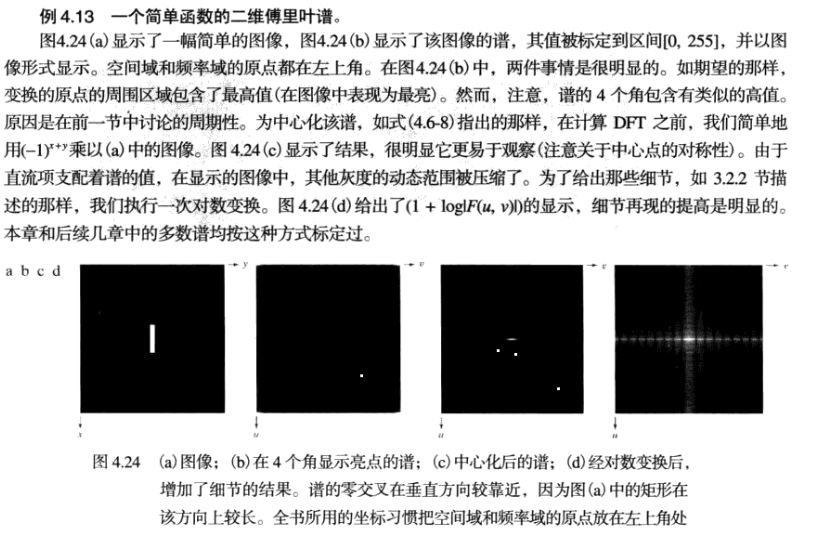
\includegraphics[width=\linewidth]{fig/fourier_spectrum.png}
\end{figure}

\textbf{相角对形状起着决定性作用!灰度信息则由谱携带。}
\begin{figure}[H]
\centering
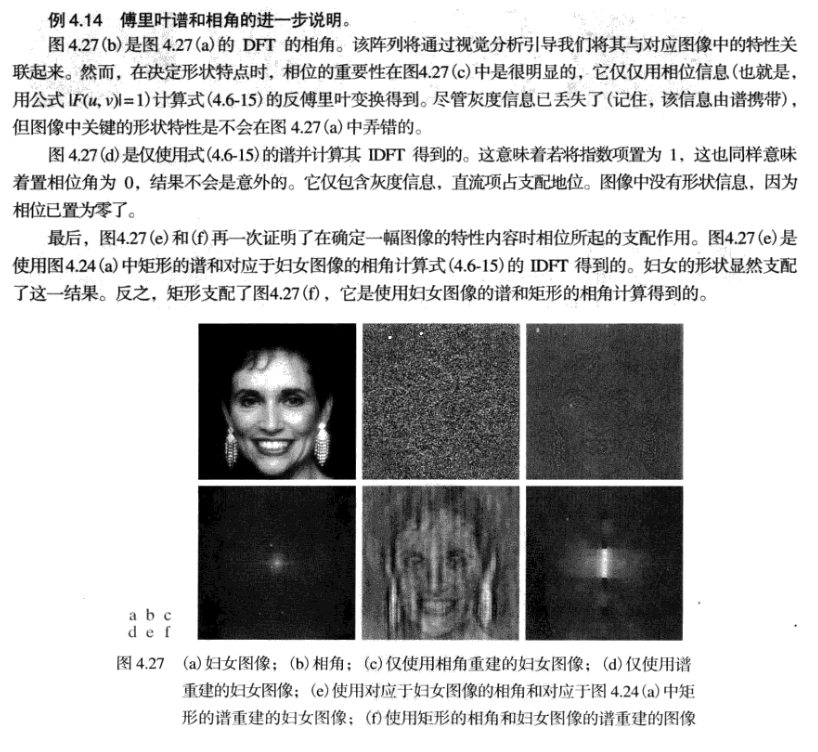
\includegraphics[width=\linewidth]{fig/spectrum_angle_example.png}
\end{figure}

\begin{theorem}[二维卷积定理]
二维的卷积定义如下
\[f(x,y)*h(x,y)=\sum_{m=0}^{M-1}\sum_{n=0}^{N-1}f(m,n)h(x-m,y-n)\]
同样有傅里叶变换对
\[\begin{aligned}
f(x,y)*h(x,y)\iff F(u,v)H(u,v)\\
f(x,y)h(x,y) \iff F(u,v)*H(u,v)
\end{aligned}\]
\end{theorem}
注意周期靠近会导致互相干扰而导致缠绕错误,因此需要进行零延拓(padding)。

假设函数$f(x)$和$h(x)$分别有$A$个和$B$个点组成,对这两个函数同时添加零,使其具有相同的周期
\[f_e=\begin{cases}
f(x) & 0\leq A-1\\
0 & A\leq x\leq P
\end{cases}
\qquad
h_e=\begin{cases}
h(x) & 0\leq x\leq B-1\\
0 & B\leq x\leq P
\end{cases}\]
同样对于二维图像滤波,若$f(x,y)$大小为$A\times B$,$h(x,y)$大小为$C\times D$,则延拓函数
\[f_e(x,y)=\begin{cases}
f(x,y) & 0\leq x\leq A-1\land 0\leq y\leq B-1\\
0 & A\leq x\leq P\lor B\leq y\leq Q
\end{cases}
\qquad
h_e(x,y)=\begin{cases}
h(x,y) & 0\leq x\leq C-1\land 0\leq y\leq D-1\\
0 & C\leq x\leq P\lor D\leq y\leq Q
\end{cases}\]
其中$P\geq A+C-1$,$Q\geq B+D-1$,通常可取$P=2M$,$Q=2N$。

\begin{definition}[相关]
相关性相当于算内积
\[g(x,y)=f(x,y)\circ h(x,y)=\sum_{m=0}^{M-1}\sum_{n=0}^{N-1}f^\star(m,n)h(x+m,y+n)\]
\end{definition}
\begin{theorem}[相关定理]
\[\begin{aligned}
f(x,y)\circ h(x,y)&\iff F^\star(u,v)H(u,v)\\
f^\star(x,y)h(x,y)&\iff F(u,v)\circ H(u,v)
\end{aligned}\]
\end{theorem}


\subsection{频率域滤波}
之所以要到频率域做滤波,是因为直观且计算比空间滤波容易(卷积耗时)
\begin{itemize}
\item 低通滤波器:平滑/模糊图像,设$D(u,v)$为频率域中点$(u,v)$与频率矩形中心的距离,$D_0$为截止频率
\begin{center}
\begin{tabular}{c|c|c}\hline
理想(ILPF) & $n$阶布特沃斯(BLPF) & 高斯\\\hline
$H(u,v)=\begin{cases}1 & D(u,v)\leq D_0\\0 & D(u,v)>D_0\end{cases}$ &
$H(u,v)=\dfrac{1}{1+[D(u,v)/D_0]^{2n}}$ &
$H(u,v)=\ee^{-D^2(u,v)/2D_0^2}$\\\hline
\end{tabular}
\end{center}
原点在频率中心,半径为$r$的圆包含的功率为
\[\alpha=\lrp{\sum_u\sum_v \frac{P(u,v)}{P_T}}\times 100\%=\lrp{\sum_u\sum_v \frac{P(u,v)}{\sum_{u=0}^{M-1}\sum_{v=0}^{N-1}|F(u,v)|^2}}\times 100\%\]
由于截止频率点处跳变太直接,物理无法实现,故是理想滤波器;而且会产生滤波模糊和振铃现象。
一阶BLPF没有振铃,二阶BLPF振铃很小,随着阶数增高振铃增大,故通常用二阶。
\item 高通滤波器:$H_{hp}(u,v)=1-H_{lp}(u,v)$,锐化图像(噪声、边缘、细节),只获得高频特征,没有背景,留下细节
\begin{center}
\begin{tabular}{c|c|c}\hline
理想(IGPF) & $n$阶布特沃斯(BGPF) & 高斯\\\hline
$H(u,v)=\begin{cases}0 & D(u,v)\leq D_0\\1 & D(u,v)>D_0\end{cases}$ &
$H(u,v)=\dfrac{1}{1+[D_0/D(u,v)]^{2n}}$ &
$H(u,v)=1-\ee^{-D^2(u,v)/2D_0^2}$\\\hline
\end{tabular}
\end{center}
\item 拉普拉斯滤波
\[H(u,v)=-4\pi^2\lrs{(u-P/2)^2+(v-Q/2)^2}=-4\pi^2D^2(u,v)\]
前面的系数可以去掉。拉普拉斯图像由下式给出
\[\nabla^2f(x,y)=\Im^{-1}[H(u,v)F(u,v)]\]
图像增强可以由下式实现
\[g(x,y)=f(x,y)+c\nabla^2 f(x,y)\]
\item 高频增强滤波:锐化/加强图像,高频增强,细节变得明显
\[\begin{aligned}
F_{lp}(u,v)&=H_{lp}(u,v)F(u,v)\\
F_{hp}(u,v)&=F(u,v)-F_{lp}(u,v)\\
&=(1-H_{lp}(u,v))F(u,v)\\
&=H_{hp}(u,v)F(u,v)\\
G(u,v)&=F(u,v)+F_{hp}(u,v)\\
&=(1+H_{hp}(u,v))F(u,v)
\end{aligned}\]
其中$k=1$为钝化模板,$k>1$为高提升滤波
\item 同态滤波器:高频增强,整个图像亮度又不能太亮(一片的亮度与低频有关)$\implies$抑制低频/环境光,提升高频/细节
\[f(x,y)=i(x,y)r(x,y)\]
其中$i(x,y)\in(0,\infty)$为照射分量(影响低频,一片);$0<r(x,y)<1$,反射率影响边缘/高频。
先取对数,然后再做傅里叶变换,最后记得取指数返回
\[\ln f(x,y)=\ln i(x,y)+\ln r(x,y)\]
同态滤波器
\[H(u,v)=(r_H-r_L)[1-\ee^{-c(D^2(u,v)/D_0^2)}]+r_L\]
其中$c$用于控制滤波器函数斜面的锐化,$r_L<1$,$r_H>1$
\begin{figure}[H]
\centering
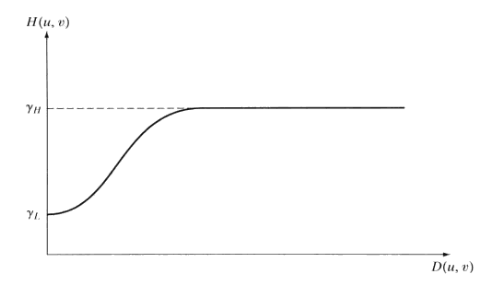
\includegraphics[width=0.4\linewidth]{fig/homo_filter.png}
\end{figure}
\end{itemize}

频率域滤波的步骤
\begin{figure}[H]
\centering
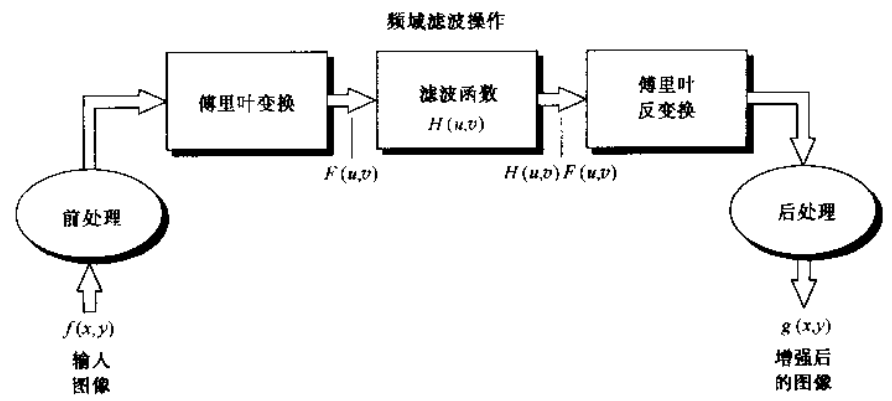
\includegraphics[width=0.6\linewidth]{fig/filter_pass.png}
\end{figure}
\begin{enumerate}
	\item 给定大小为$M\times N$的输入图像$f(x,y)$,选择填充参数$P=2M$,$Q=2N$
	\item 对$f(x,y)$添加必要的0,形成大小为$P\times Q$的填充后的图像$f_p(x,y)$
	\item 用$(-1)^{x+y}$乘以$f_p(x,y)$,做频谱中心化处理
	\item 用上面结果计算DFT,得到$F(u,v)$
	\item 生成一个\textbf{实对称}的滤波函数$H(u,v)$,大小为$P\times Q$,中心在$(P/2,Q/2)$处。
	用阵列相乘得到$G(u,v)=H(u,v)F(u,v)$
	\item 计算上式得到的IDFT,并恢复原图像
	\[g_p(x,y)=\Real[\Im[G(u,v)]](-1)^{x+y}\]
	\item 通过从$g_p(x,y)$的左上角提取$M\times N$大小的区域,得到最终结果$g(x,y)$
\end{enumerate}

\subsection{总结}
傅里叶变换的一些性质
\begin{itemize}
	\item 线性性:
	\[af_1(x,y)+bf_2(x,y)\iff aF_1(u,v)+bF_2(u,v)\]
	\item 平移性质:
	\[\begin{aligned}
	&f(x,y)\ee^{j2\pi(u_0x/M+v_0y/N)}\iff F(u-u_0,v-v_0)\\
	&f(x-x_0,y-y_0)\iff F(u,v)\ee^{-2j\pi(x_0u/M+y_0v/N)}
	\end{aligned}\]
	特别地,平移到频率矩形中心$(M/2,N/2)$
	\[\begin{aligned}
	&f(x,y)(-1)^{x+y}\iff F(u-M/2,v-N/2)\\
	&f(x-M/2,y-N/2)\iff F(u,v)(-1)^{u+v}
	\end{aligned}\]
	\item 旋转性质:使用极坐标$x=r\cos\theta,y=r\sin\theta,u=\omega\cos\varphi,v=\omega\sin\varphi$,有
	\[f(r,\theta+\theta_0)\iff F(\omega,\varphi+\varphi_0)\]
	\item 周期性:
	\[\begin{aligned}
	F(u,v)&=F(u+k_1M,v+k_2N)\\
	f(x,y)&=f(x+k_1M,y+k_2N)
	\end{aligned}\]
	\item 对称性:
	实函数$f(x,y)$的傅里叶变换是共轭对称/哈密特对称的
	\[F^\star(u,v)=F(-u,-v)\]
	而虚函数$f(x,y)$的傅里叶变换是共轭反对称的
	\[F^\star(-u,-v)=-F(u,v)\]
	\item 可分性:2D-FFT可变成两个1D-FFT
	\[F(u,v)=\sum_{x=0}^{M-1}\lrp{\sum_{y=0}^{N-1}f(x,y)\ee^{-j2\pi ux/M}}\ee^{-j2\pi vy/N}\]
\end{itemize}

常见函数的傅里叶变换
\begin{center}
\begin{tabular}{|c|l|}\hline
离散单位冲激 & $\delta(x,y)\iff 1,\;1\iff\delta(u,v)$\\\hline
矩形函数 & $\mathrm{rect}[a,b]\iff ab\frac{\sin(\pi ua)}{\pi ua}\frac{\sin(\pi ub)}{\pi ub}\ee^{-j\pi(ua+vb)}$\\\hline
正弦函数 & $\sin(2\pi u_0x+2\pi v_0y)\iff j\frac{1}{2}[\delta(u+Mu_0,v+Nv_0)-\delta(u-Mu_0,v-Nv_0)]$\\\hline
余弦函数 & $\cos(2\pi u_0x+2\pi v_0y)\iff j\frac{1}{2}[\delta(u+Mu_0,v+Nv_0)+\delta(u-Mu_0,v-Nv_0)]$\\\hline
微分 & $\frac{\diff^n f(x)}{\diff x^n}\iff (ju)^n F(u),\;\lrp{\pd{}{t}}^m\lrp{\pd{}{z}}^nf(t,z)\iff(j2\pi u)^m(j2\pi v)^nF(u,v)$\bigstrut\\\hline
高斯 & $A2\pi\sigma^2\ee^{-2\pi^2\sigma^2(t^2+z^2)}\iff A\ee^{-(u^2+v^2)/2\sigma^2}$\\\hline
\end{tabular}
\end{center}

用前向变换计算傅里叶反变换,以消除两套冗余电路
\[MNf^\star(x,y)=\sum_{u=0}^{M-1}\sum_{v=0}^{N-1} F^\star(u,v)\ee^{-j2\pi (ux/M+vy/N)}\]

\end{document}